\section{Storia del filtraggio e principali problemi affrontati}

L'essere umano, da sempre, sfrutta i propri sensi per relazionarsi con il mondo.\\
Il suo primo riferimento in particolare è la vista, senza la quale egli si sente perso, smarrito; per questo è fondamentale sviluppare un linguaggio  visivo che sia efficace.\\
La società contemporanea sfrutta immagini di vario genere (fotografie, radiografie, ecografie, poster pubblicitari, progetti, etc.) per comunicare messaggi e/o per rendere chiari progetti, idee, situazioni.\\
\`E quindi un problema sempre di grande interesse cercare di sfruttarle al meglio. A tal proposito esistono alcuni metodi di \textbf{filtraggio}, la cui finalità è quella di migliorare la qualità delle immagini, metterne in risalto determinate caratteristiche o nasconderne delle altre.\\


\subsection{Filtraggio analogico}
Anche prima dell'avvento dei computer esisteva l'elaborazione delle immagini. Esistevano infatti dei procedimenti, detti \textit{"mascherature"}, che servivano a ridurre o esaltare le differenze di luce nella foto.\\
La mascheratura avveniva durante la fase di stampa su carta, ossia quando il negativo veniva proiettato sulla carta fotografica mediante l’ingranditore.\\

\noindent
Qui, %lo “stampatore” 
l'operatore utilizzava una serie di metodi per far sì che su certe zone della carta andasse più o meno luce di quella che sarebbe arrivata passando attraverso il negativo.\\

\noindent
Ad esempio la tecnica nota come \textit{"altissimo contrasto"} permetteva di avere foto con soli bianchi e soli neri, il viraggio invece serviva a dare un tono di colore alla foto, che restava comunque un bianco e nero: famoso il viraggio tono seppia.\\
\newpage


\subsection{Immagini digitali}
\cite{storia}\\
Le immagini digitali trovarono le prime applicazioni sui giornali negli anni 20. Non esistevano veri e propri computer, il segnale era trasmesso tramite telegrafo simulando dei mezzitoni.
In particolare, il sistema di trasmissione di immagini via cavo Bartlane era una tecnica inventata nel 1920 per trasmettere immagini di giornali digitalizzate su linee sottomarine tra Londra e New York.\\
Il sistema di trasmissione di immagini via cavo Bartlane generava sia sul trasmettitore che sul ricevitore una scheda dati perforata o un nastro che veniva ricreato come immagine.\\

\begin{figure}[htb] \centering
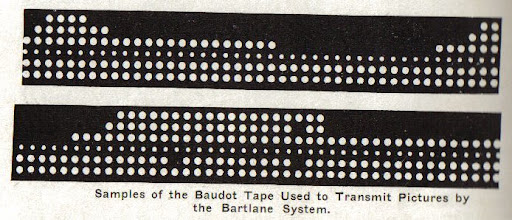
\includegraphics[scale=0.7, trim = 0 1.1cm 0 0, clip]{Pictures/nastro Bartlane.jpg}
\caption{Nastro dati codificante un'immagine.}\label{fig:figura}
\end{figure}


In questo modo riusciva a codificare immagini in bianco e nero in cinque diverse gradazioni di grigio, capacità poi ampliata a 15 gradazioni nel 1929.

\begin{figure}[htb] \centering
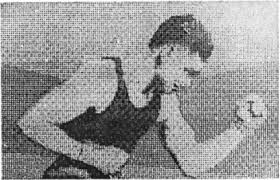
\includegraphics[scale=0.5, trim = 0 1.1cm 0 0, clip]{Pictures/img del 1921 a 5 gradazioni di grigio.jpg}
\qquad\qquad
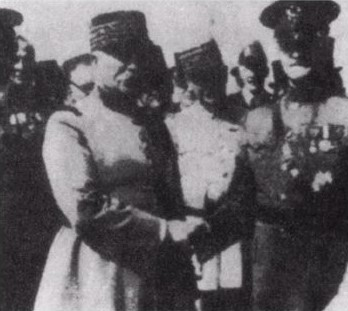
\includegraphics[scale=1.7, trim = 0 1.1cm 0 0, clip]{Pictures/img del 1929 a 15 gradazioni di grigio.jpg}
\caption{La prima immagine risale al 1921 ed è composta da 5 gradazioni di grigio.\\ 
La seconda è del 1929 ed è composta da 15 gradazioni di grigio.}\label{fig:figura}
\end{figure}
\vspace{1em} \noindent
Questa, in qualche modo, è la nascita delle immagini digitali, anche se non sono trattate da computer e quindi codificate in maniera differente. Inoltre in questa fase non abbiamo una vera e propria elaborazione delle immagini, ma solo una trasmissione e la successiva stampa.

\vspace{1em} \noindent
Nel 1957, Russell A. Kirsch produsse un dispositivo che generava dati digitali che potevano essere archiviati in un computer; questo utilizzava uno scanner a tamburo e un tubo fotomoltiplicatore.\\
Negli anni immediatamente successivi, tale invenzione portò a notevoli sviluppi.


\subsection{Filtraggio digitale}
\cite{storia}
Nel 1960 presso il Jet Propulsion Laboratory, il Massachusetts Institute of Technology, i Bell Laboratories, l'Università del Maryland, e altre strutture di ricerca svilupparono molte delle tecniche di elaborazione digitale di immagini (o della trasformazione di immagini digitali come spesso veniva chiamata) al fine di evitare le debolezze operative delle fotocamere a pellicola per missioni scientifiche e militari.\\
Queste trovarono poi applicazione in immagini satellitari, immagini medicali, videocitofono, riconoscimento ottico dei caratteri, e miglioramenti fotografici.

Il costo dell'elaborazione in quel periodo era piuttosto alto con l'apparecchiatura di elaborazione. Le cose cambiarono negli anni settanta, quando computer più economici e hardware dedicato furono resi disponibili sul mercato.\\
Le immagini allora potevano essere elaborate in tempo reale, l'elaborazione digitale sostituisce così i vecchi metodi a pellicola per molti scopi.\\

\vspace{1em}
Negli anni 2000, grazie all'avvento di computer più veloci, l'elaborazione delle immagini digitali diventò la forma più comune di elaborazione delle immagini e, in generale, divenne il metodo più utilizzato data la sua versatilità e il basso costo.

La tecnologia di elaborazione delle immagini digitali per applicazioni mediche è stata inserita nel 1994 nella Hall of Fame della Space Foundation.\\
